% Chapter 4

\chapter{Implementation and Evaluation} % Main chapter title

\label{Chapter4} % For referencing the chapter elsewhere, use \ref{Chapter1}

\lhead{Chapter 4. \emph{Implementation and Evaluation}} % This is for the header on each page - perhaps a shortened title

%----------------------------------------------------------------------------------------
\section{Development Stages }
Following are the stages of development:
\subsection{Strategy Stage}
We designed our web application while keeping in mind the requirements of our end sellers and customers. In order to make it a success we planned each and everything beforehand. We have learned our users demand and then planned our project on it. We have designed it in such a way that it can be easy to use and handle. After jotting down our requirements we made diagrams so that it can give an outlook of our system. After this we worked on our database and later on its implementation. We also wrote the project code, then we integrated and tested our it to verify if its working.

\section{Implementation}
Following is described about the implementation level things:

\subsection{Tools and Technologies}
\begin{enumerate}
	\item Server-Side API Framework \textbf{Ruby on Rails}
	\item Front-End Frameworks:
	\begin{itemize}
		\item \textbf{Next.js} (framework built on REACT Js library)
		\item \textbf{Bootstrap5} (CSS framework)
		\item \textbf{Google Material UI} (for interactive components)
		\item \textbf{Google Maps API}
	\end{itemize}
	\item DBMS \textbf{PostgreSQL}
	\item Version Control System (VCS): \textbf{Git, Github}
	\item Integrated Development Environment (IDE): \textbf{RubyMine, VS Code}
	\item API and Web testing tool: \textbf{Postman}
	\item Data Caching server: \textbf{Redis}
	\item Hosting Service for API: \textbf{Heroku}
	\item Hosting Service for Front-End App: \textbf{Amazon Static Hosting S3}
	\item CI | CD tool: \textbf{Github Actions}
	\item Media Storage Service: \textbf{AWS S3}
	\item Image Recognition Service: \textbf{AWS Rekognition}
	\item Domain Name Service: \textbf{AWS Route53}
	\item Domain Platform: \textbf{Namecheap.me}
	\item Bug Report Service: \textbf{Sentry}
	\item Mailer Service: \textbf{Mailjet}
	
\end{enumerate}

\section{System Integration}
System integration in the "Track My Shop" project is a critical process where all the individual components and modules of the system are combined and tested to ensure they function as a unified, cohesive unit. This integration involves merging the backend functionalities, including database management and server operations, with the frontend user interface to create a seamless and functional application. The integration process also incorporates third-party services, such as image recognition, mapping APIs and Deployment on AWS/Heroku, ensuring their proper interaction within the application. Rigorous testing and validation are conducted to confirm that the integrated system operates smoothly, with data flowing seamlessly between various components.\\
Achieving a successful integration is vital for delivering a reliable, efficient, and feature-rich web application that can be run on any environment and on any web browser, meets the needs and expectations of both sellers and customers. 

\section{User Interface}
The user interface (UI) of the "Track My Shop" project is crafted to deliver a seamless and engaging experience for both sellers and customers. Sellers are provided with a comprehensive dashboard offering insights into their shops, order requests, and sales statistics. They can efficiently manage their shop listings, adding new products/services and updating existing ones. On the other hand, customers are greeted with an intuitive interface that allows effortless browsing of nearby shops and their offerings, categorized for easy exploration. The search functionality is versatile, enabling customers to search by text, images, or based on their preferences. Clear product/service details, interactive maps for shop locations, easy order request processes, and a user-friendly profile management system further enhance the overall usability. The UI is designed to be accessible and responsive to various type of devices and user needs, ultimately fostering a positive and satisfying interaction for all users.
\newpage

\begin{figure}[h]
	\subsection{Login}
	\centering
	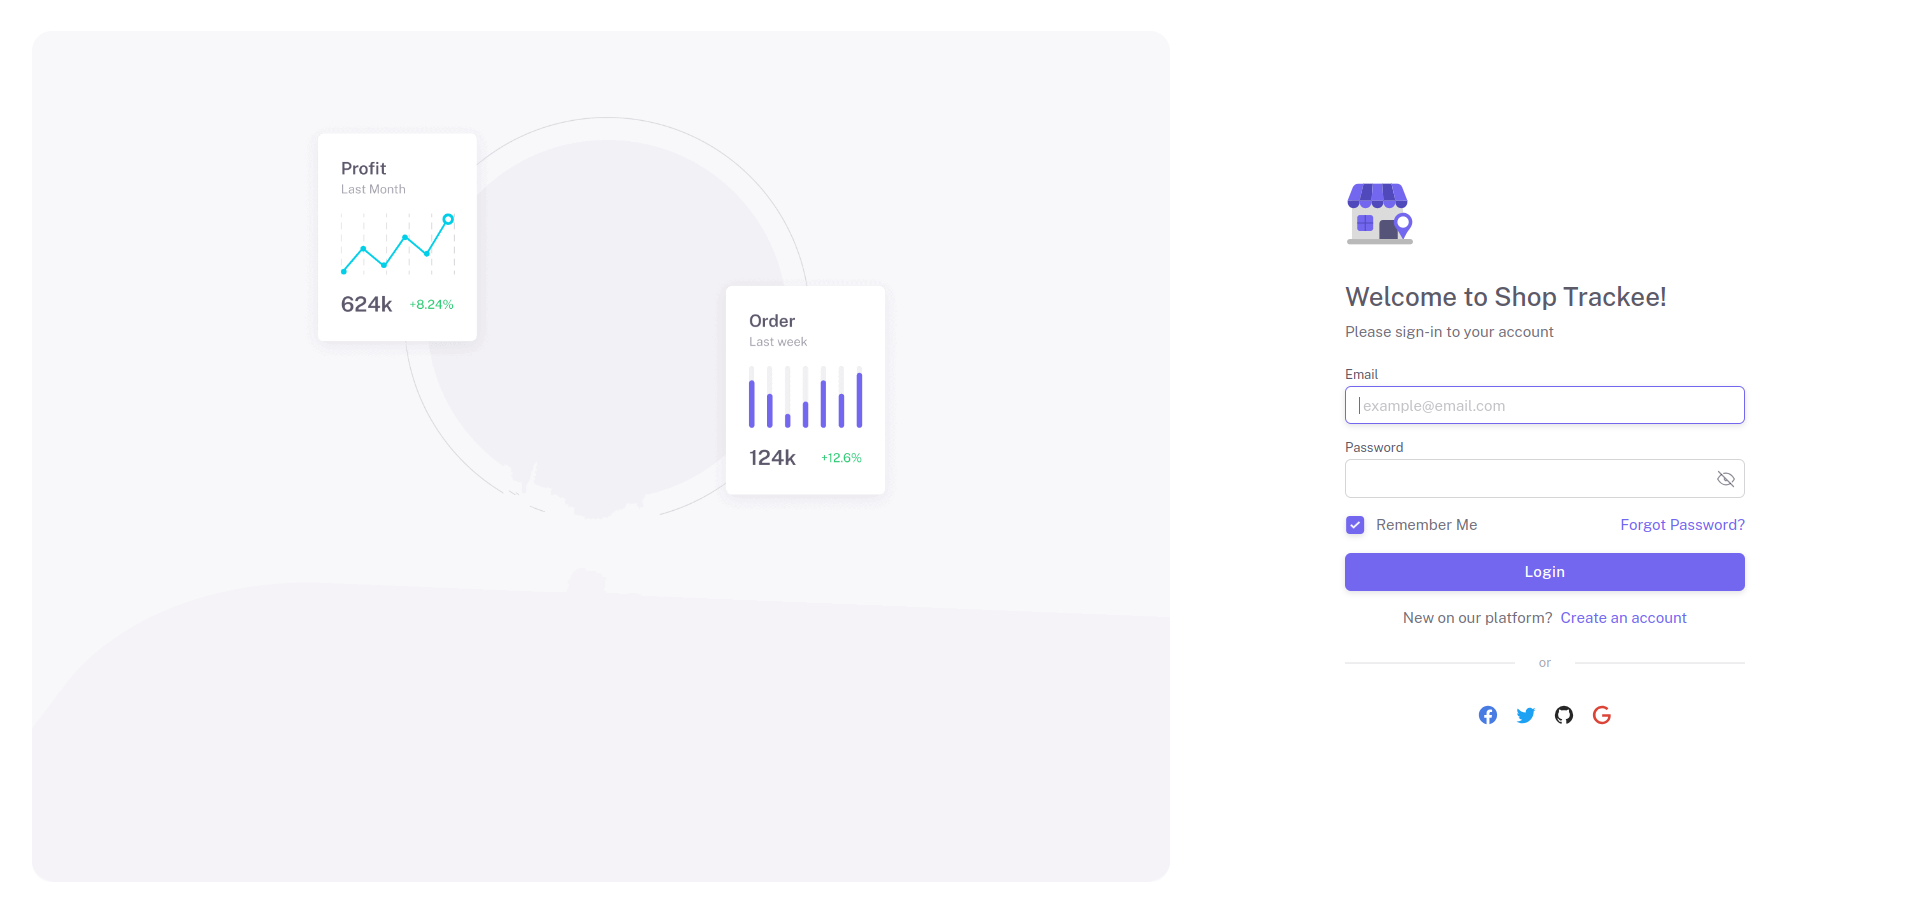
\includegraphics[width=1\textwidth]{login-page}
	\caption{Shop Trackee - Login}
\end{figure}

\begin{figure}[h]
	\subsection{Register}
	\centering
	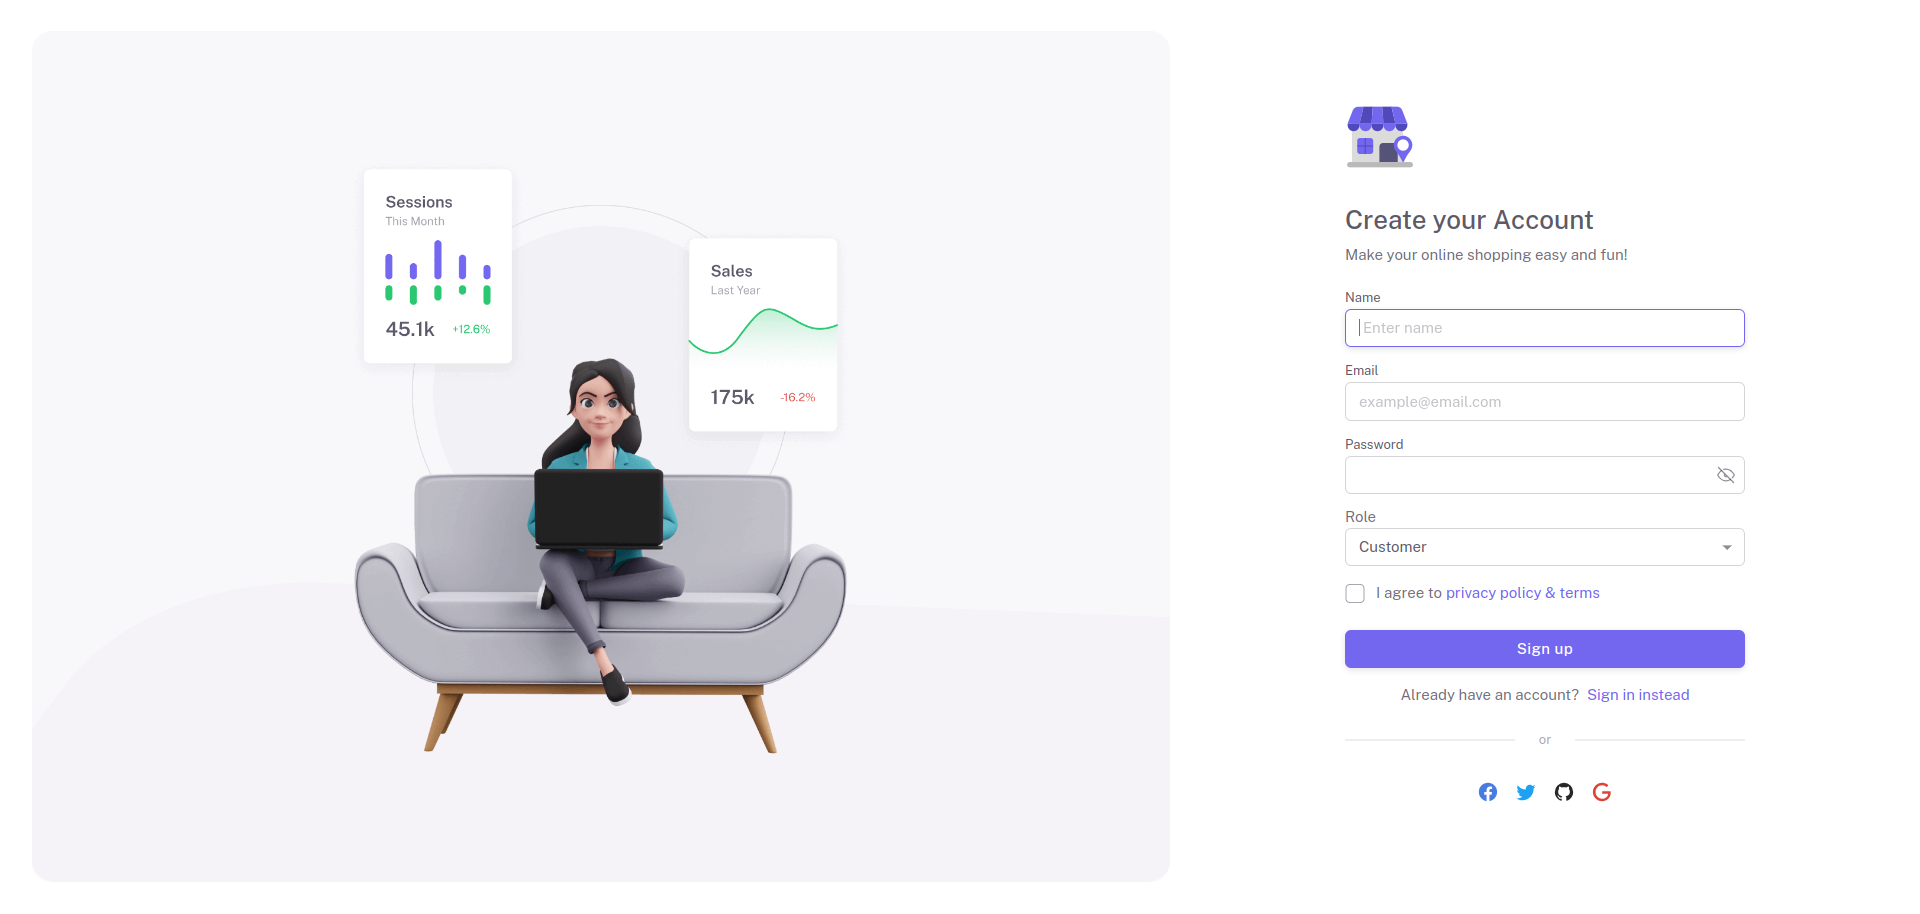
\includegraphics[width=1\textwidth]{signup-page}
	\caption{Shop Trackee - Register}
\end{figure}
\newpage

\begin{figure}[h]
	\subsection{Forgot Password}
	\centering
	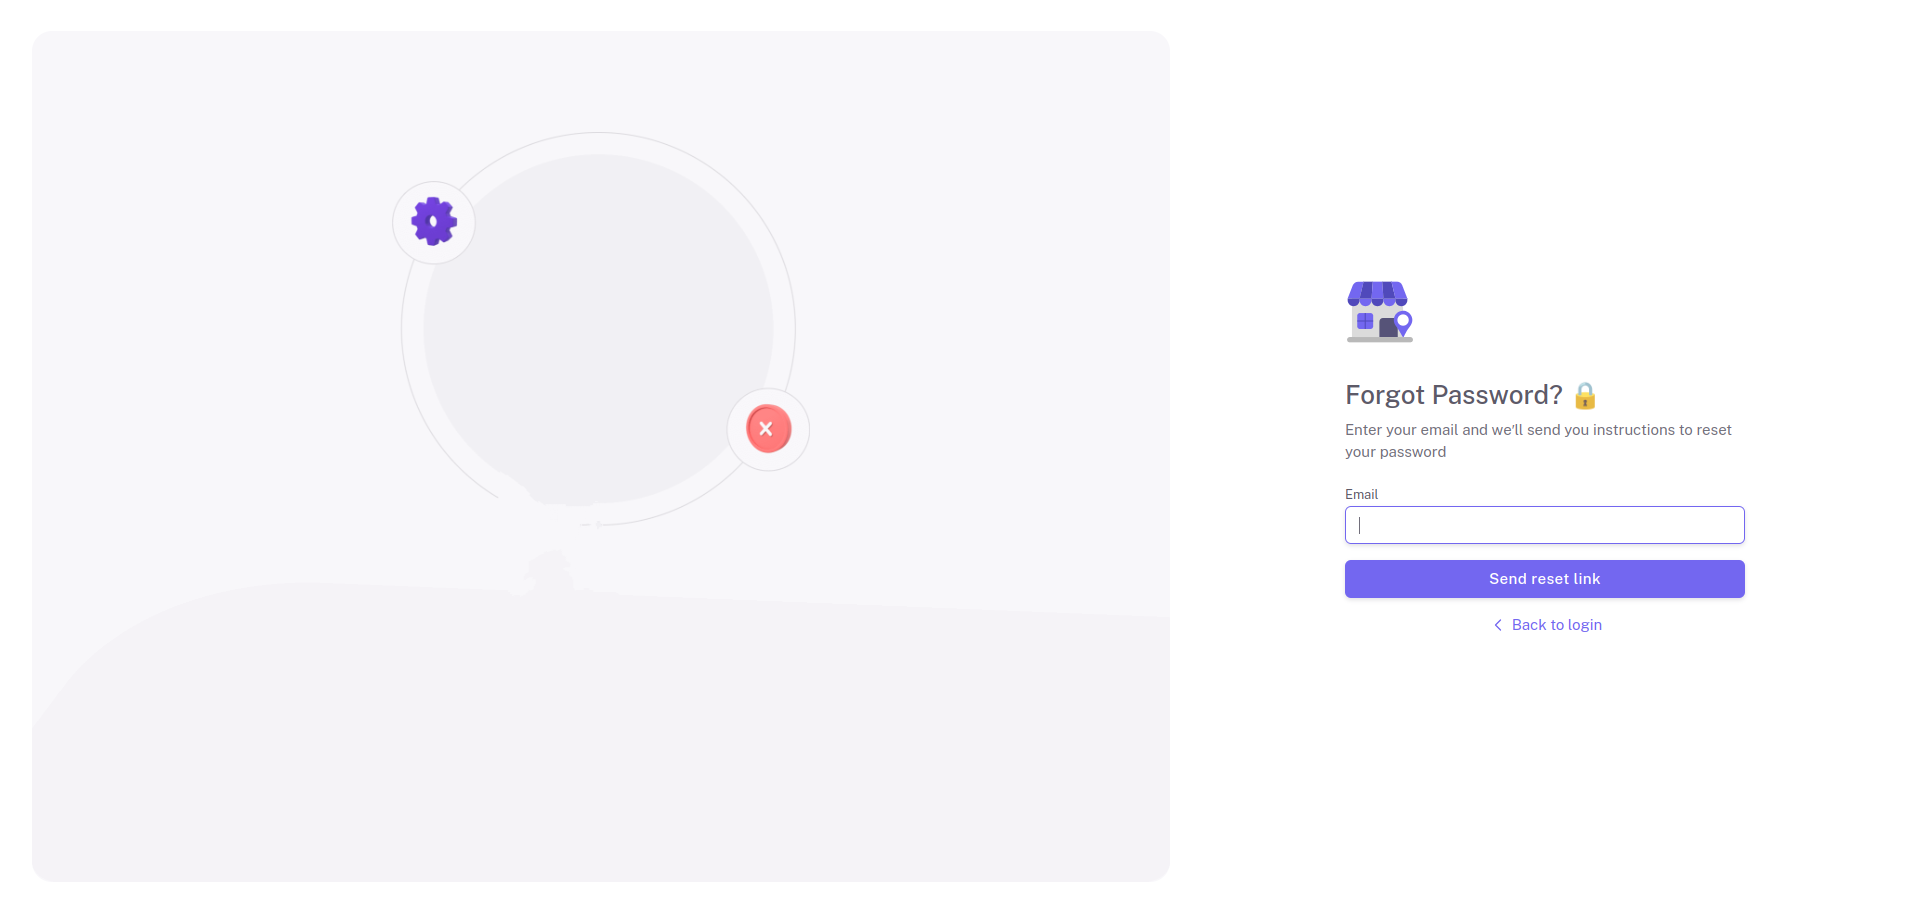
\includegraphics[width=1\textwidth]{forgot-password-page}
	\caption{Shop Trackee - Forgot Password}
\end{figure}

\begin{figure}[h]
	\subsection{Profile}
	\centering
	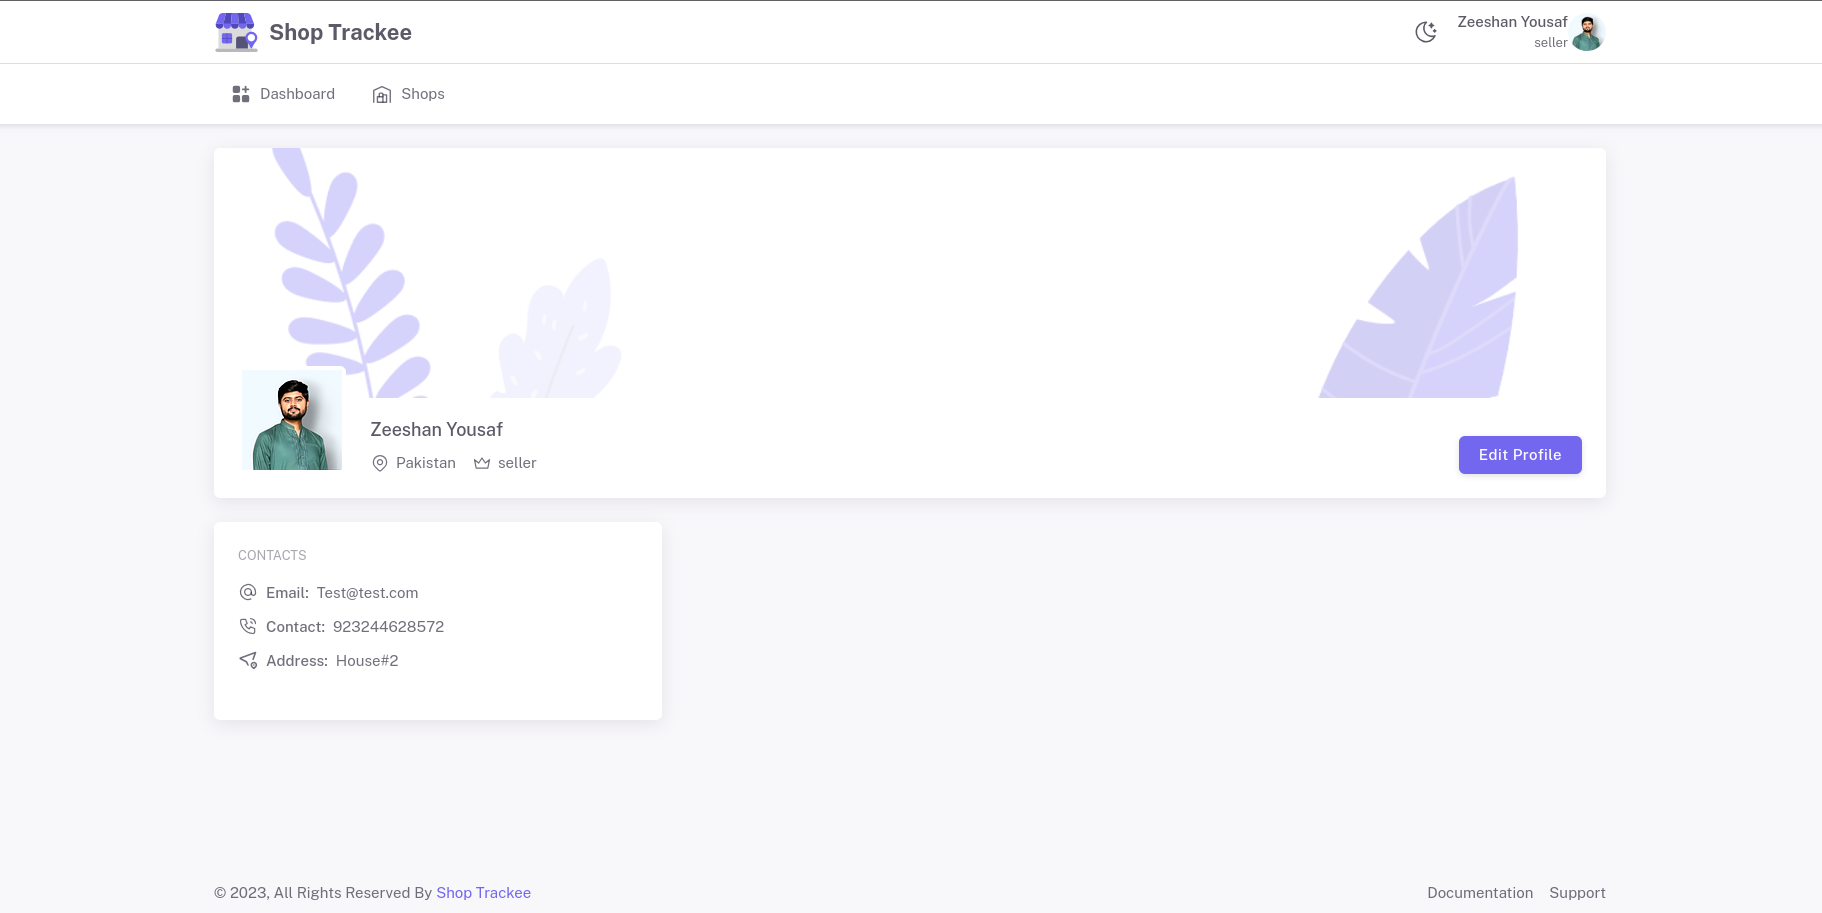
\includegraphics[width=1\textwidth]{seller-profile-page}
	\caption{Shop Trackee - Profile}
\end{figure}
\newpage

\begin{figure}[h]
	\subsection{Profile Edit}
	\centering
	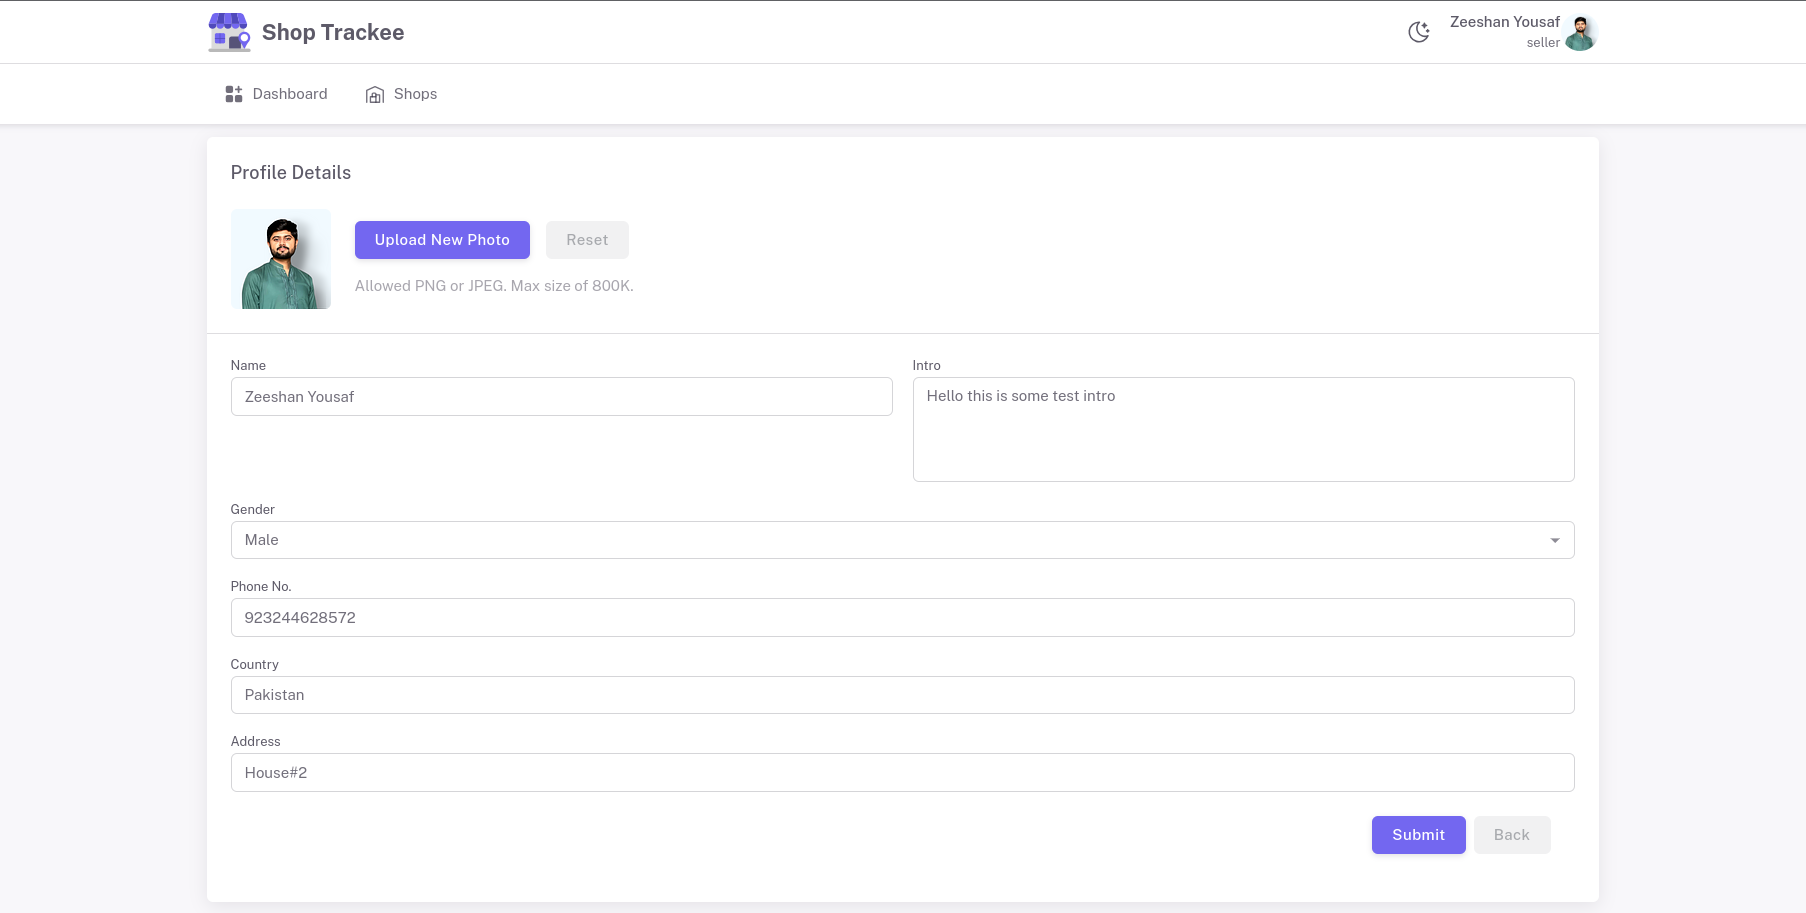
\includegraphics[width=1\textwidth]{profile-edit-page}
	\caption{Shop Trackee - Profile Edit}
\end{figure}


\begin{figure}[h]
	\subsection{Seller Dashboard}
	\centering
	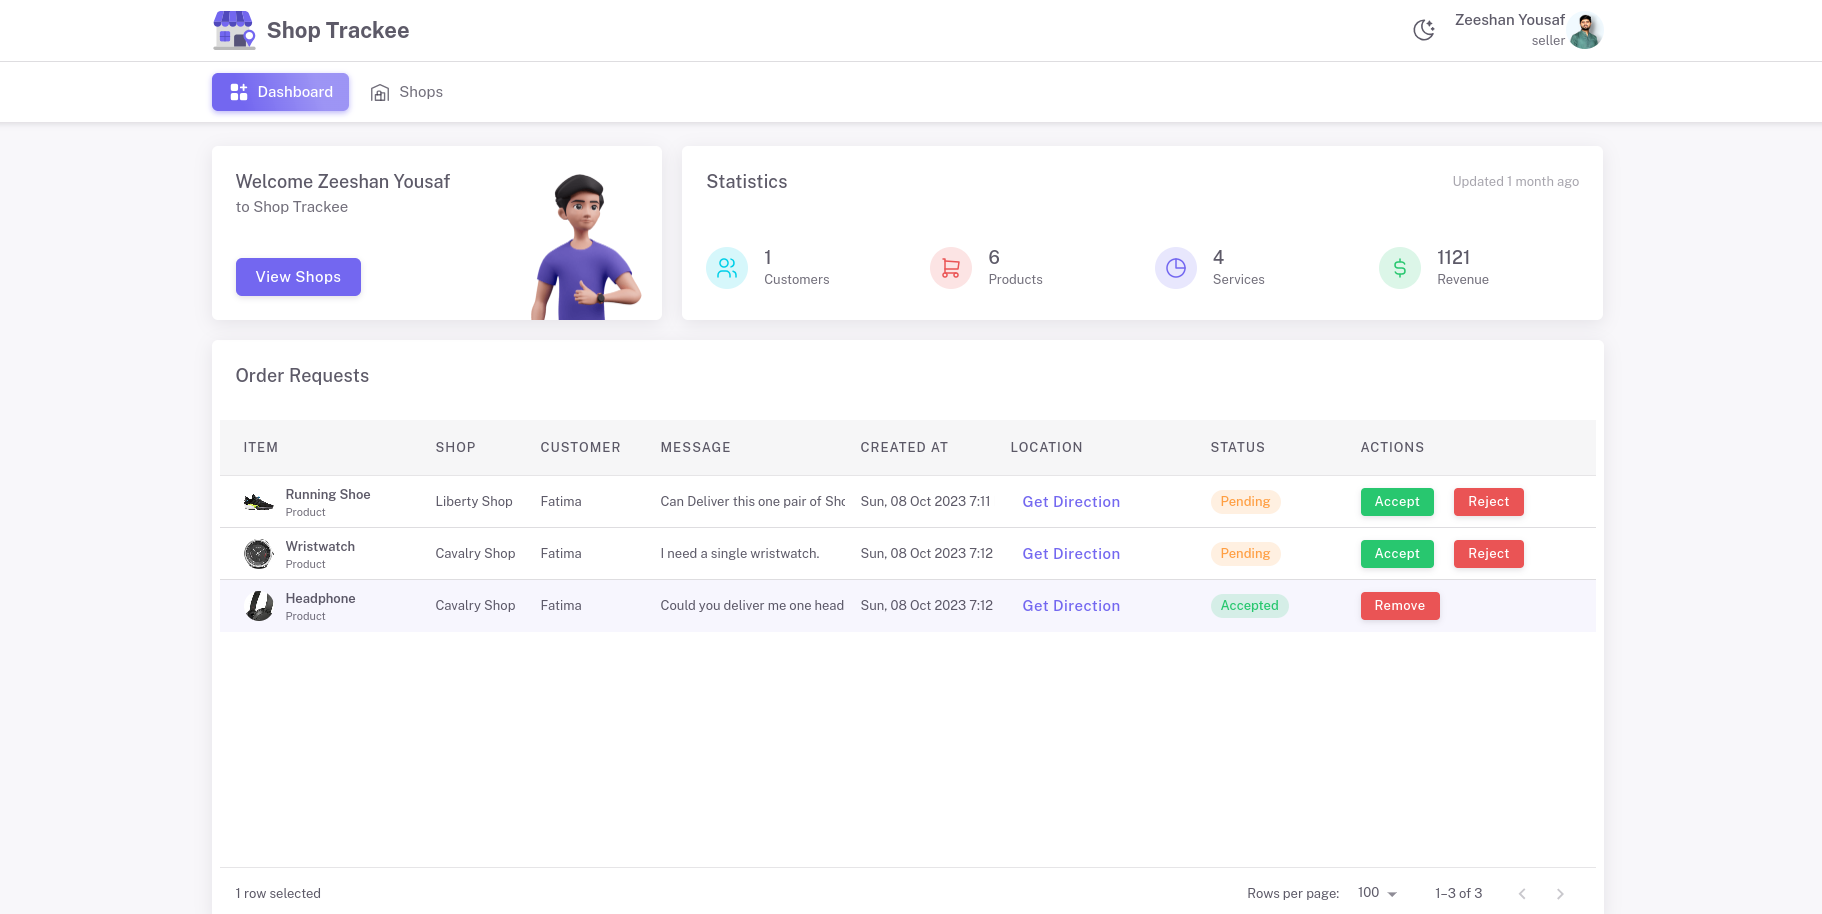
\includegraphics[width=1\textwidth]{seller-dashboard-page}
	\caption{Shop Trackee - Seller Dashboard}
\end{figure}
\newpage

\begin{figure}[h]
	\subsection{Seller Shops}
	\centering
	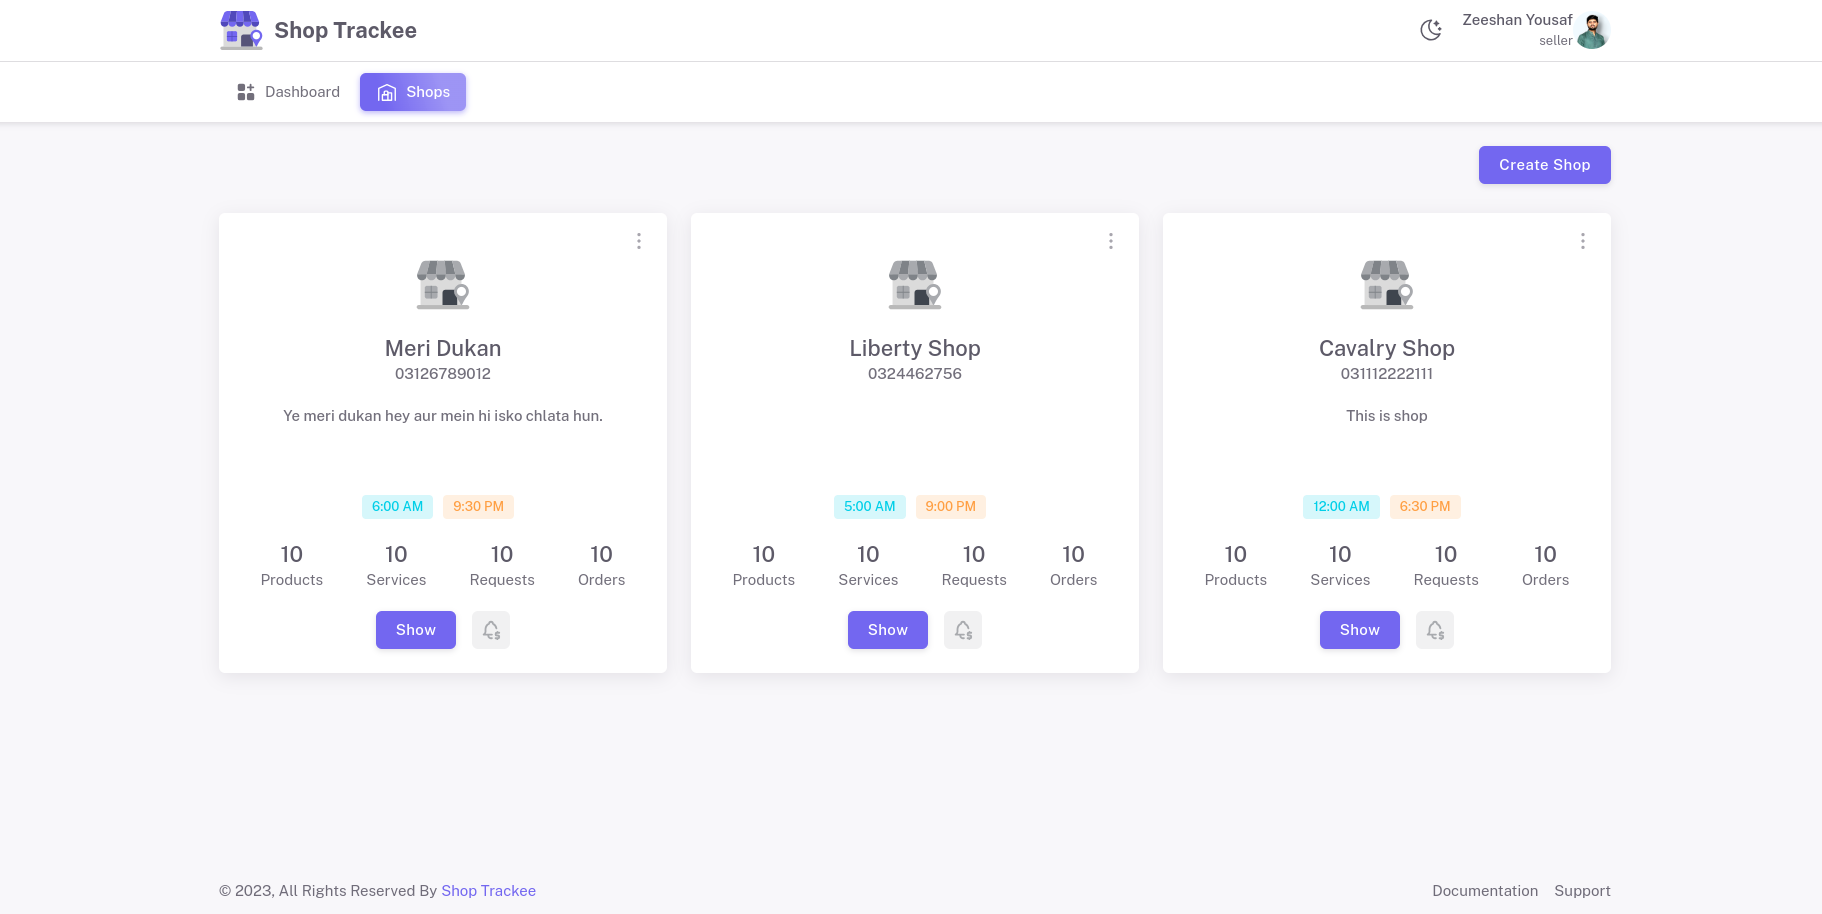
\includegraphics[width=1\textwidth]{seller-shops-page}
	\caption{Shop Trackee - Seller Shops}
\end{figure}

\begin{figure}[h]
	\subsection{Seller Shop Create}
	\centering
	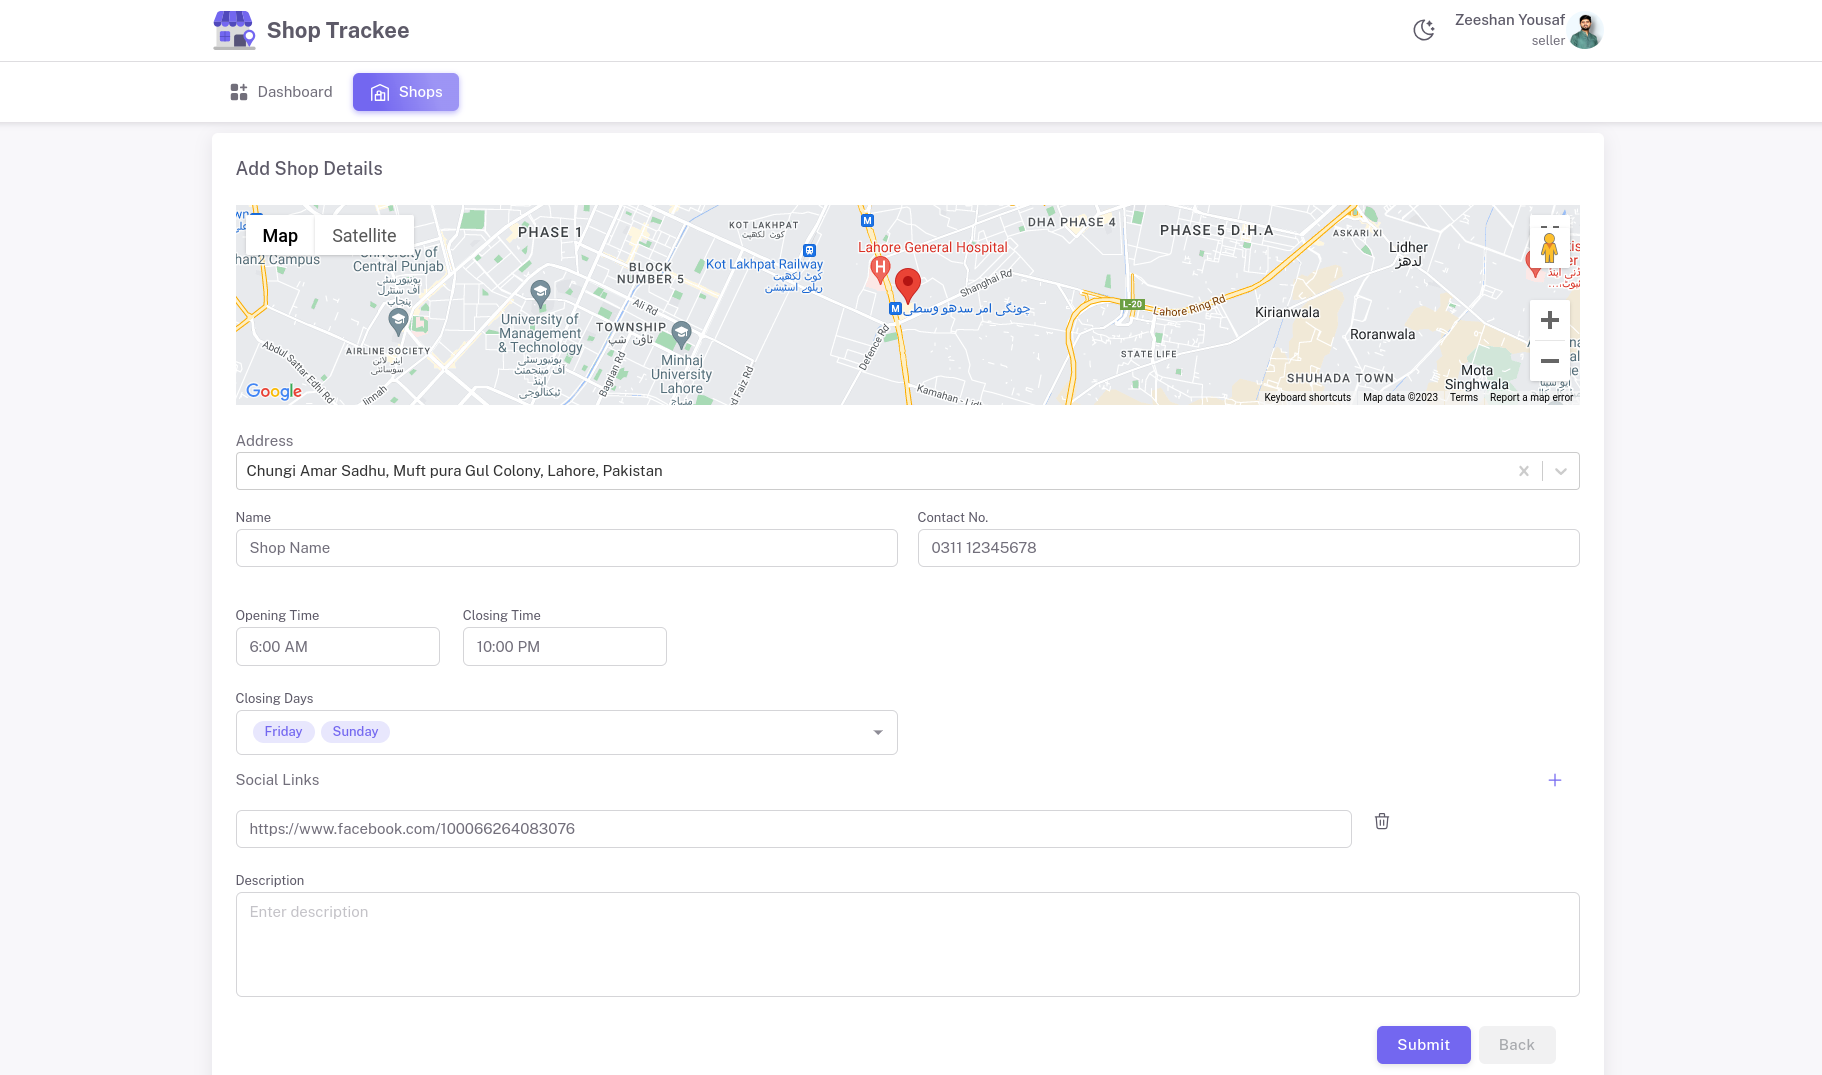
\includegraphics[width=0.9\textwidth]{seller-shop-create-page}
	\caption{Shop Trackee - Shop Create}
\end{figure}
\newpage

\begin{figure}[h]
	\subsection{Seller Add Product}
	\centering
	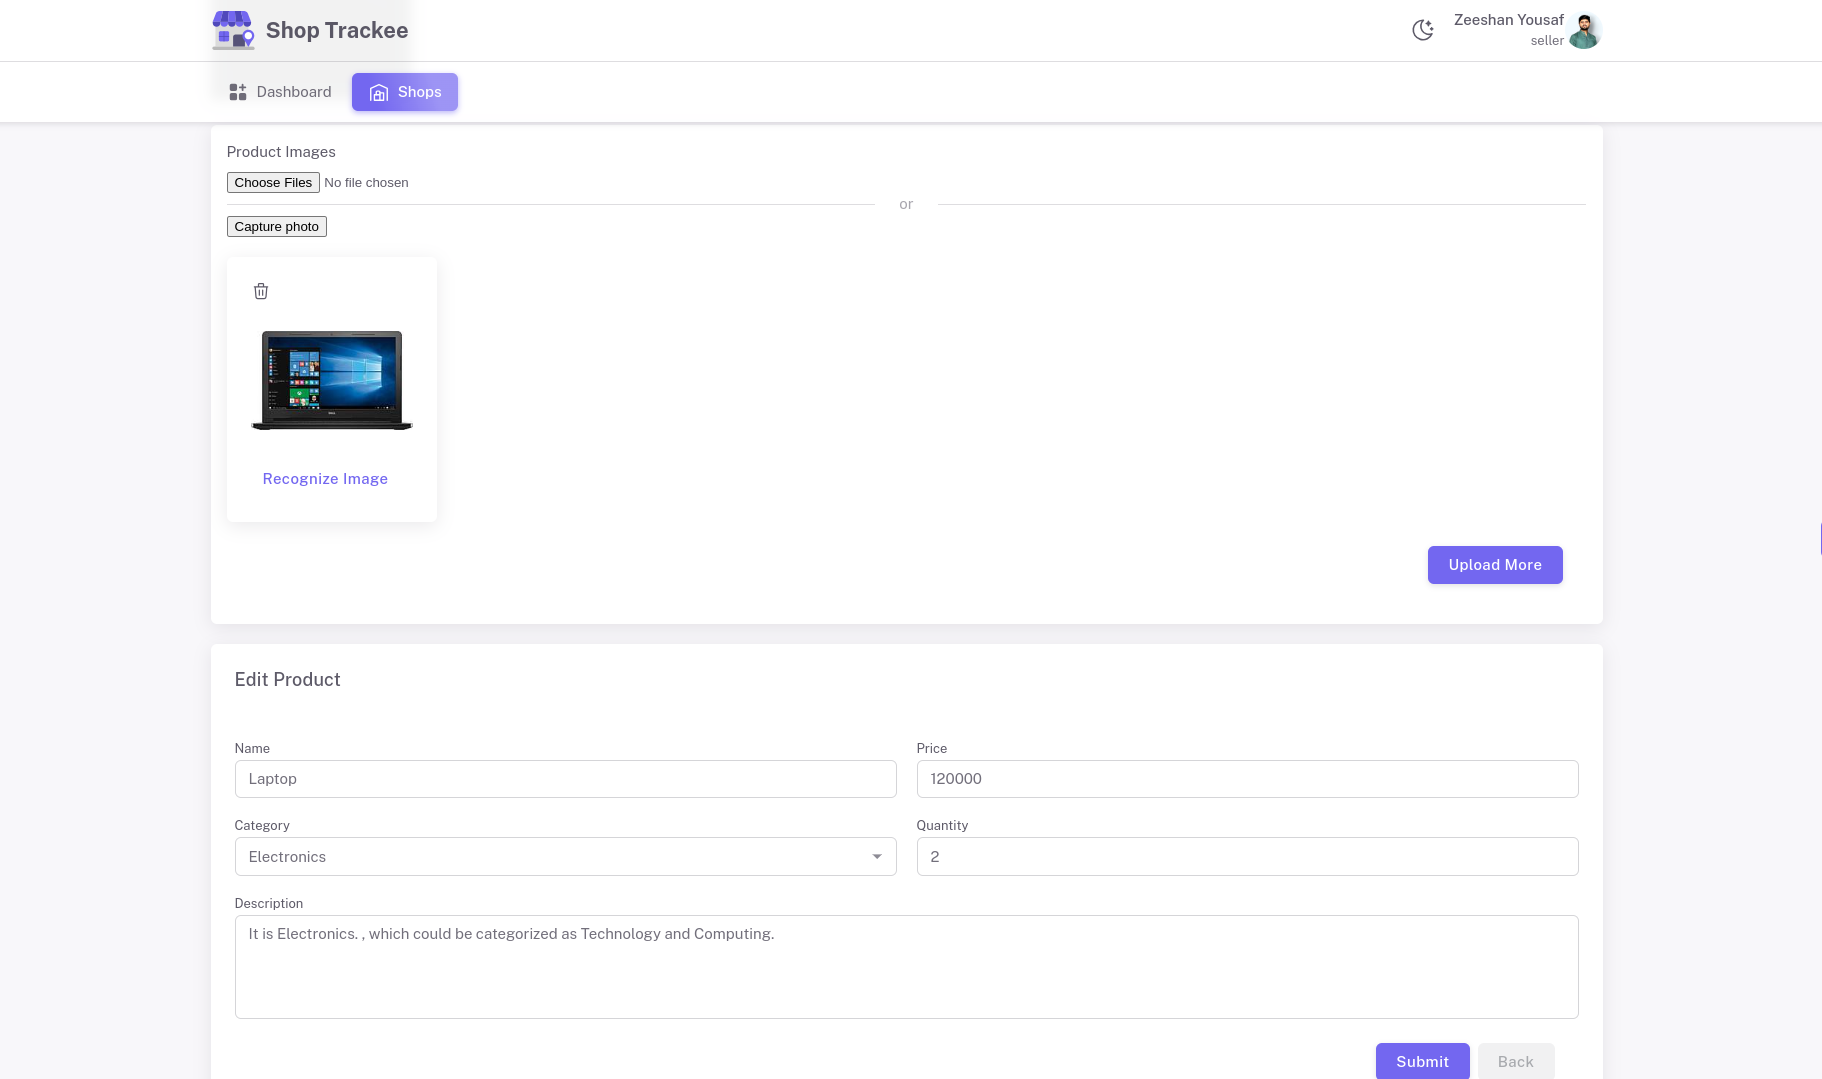
\includegraphics[width=1\textwidth]{product-form-page}
	\caption{Shop Trackee - Add Product}
\end{figure}

\begin{figure}[h]
	\subsection{Seller Add Service}
	\centering
	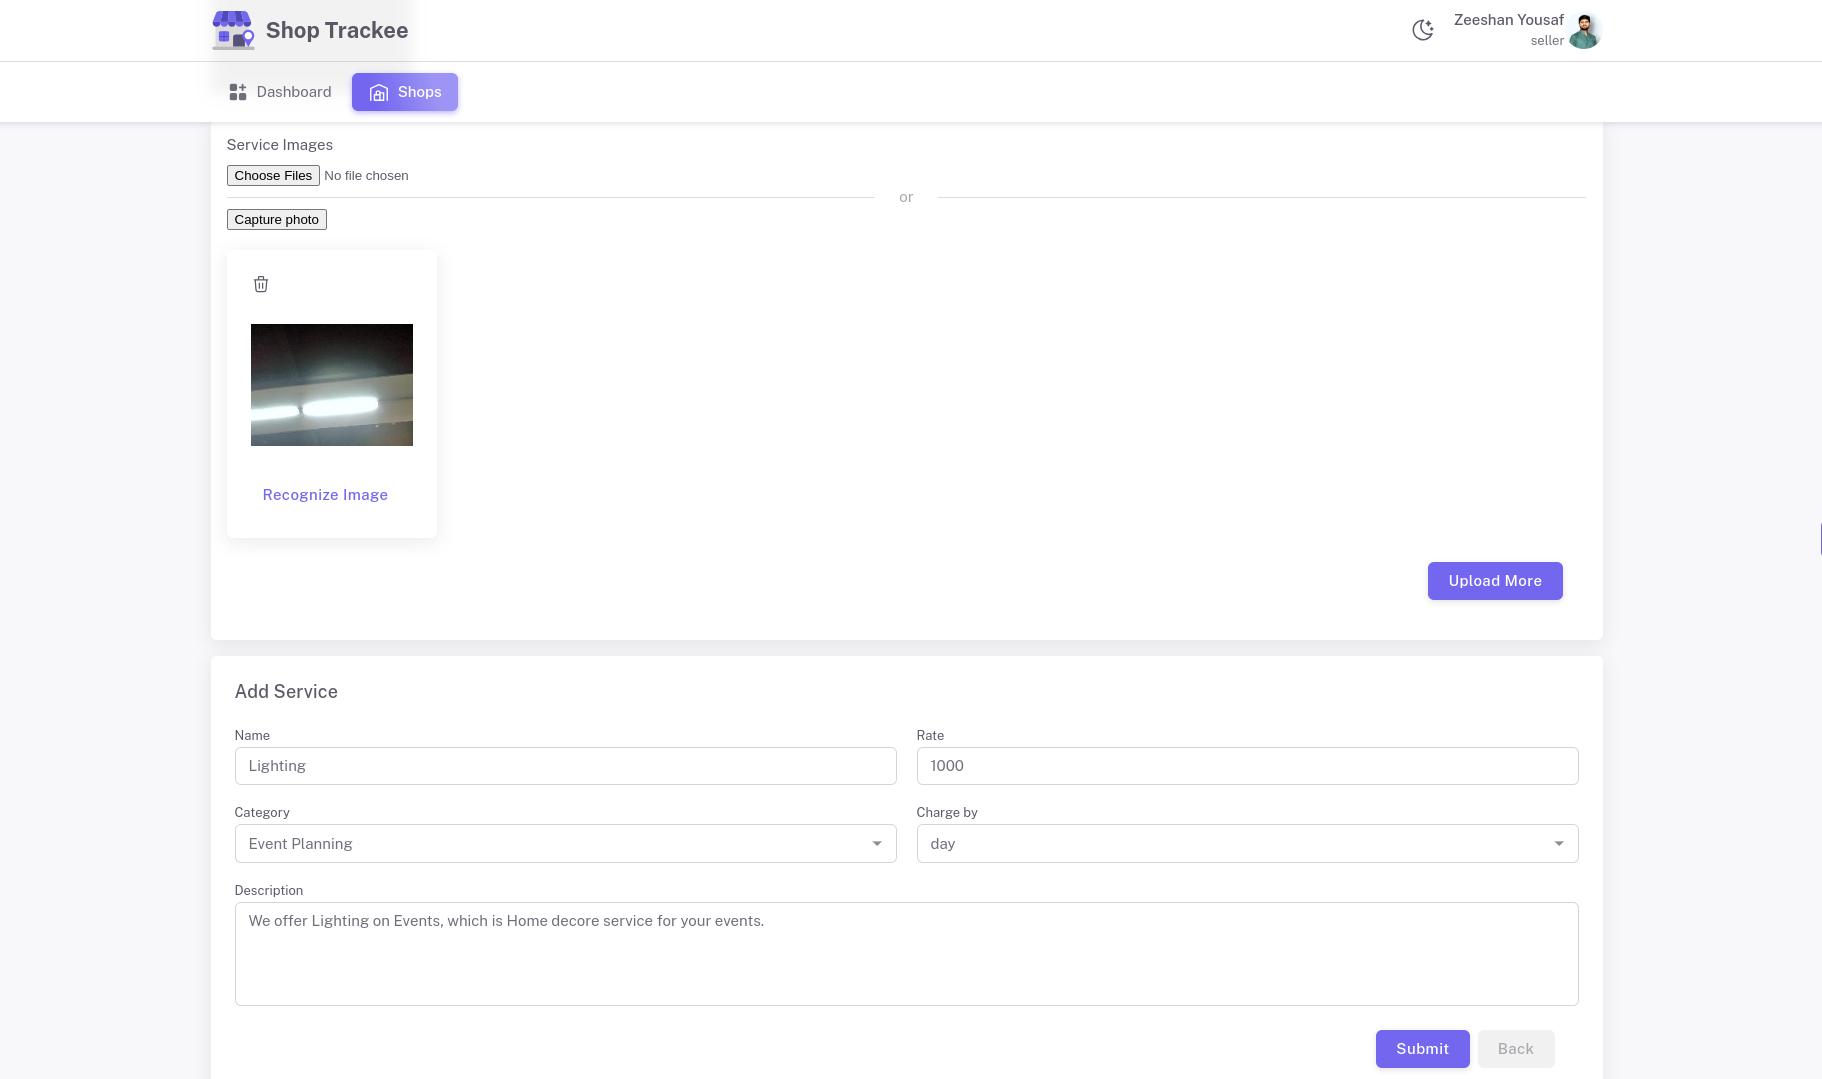
\includegraphics[width=0.9\textwidth]{service-form-page}
	\caption{Shop Trackee - Add Service}
\end{figure}
\newpage

\begin{figure}[h]
	\subsection{Seller Products and Services Listing}
	\centering
	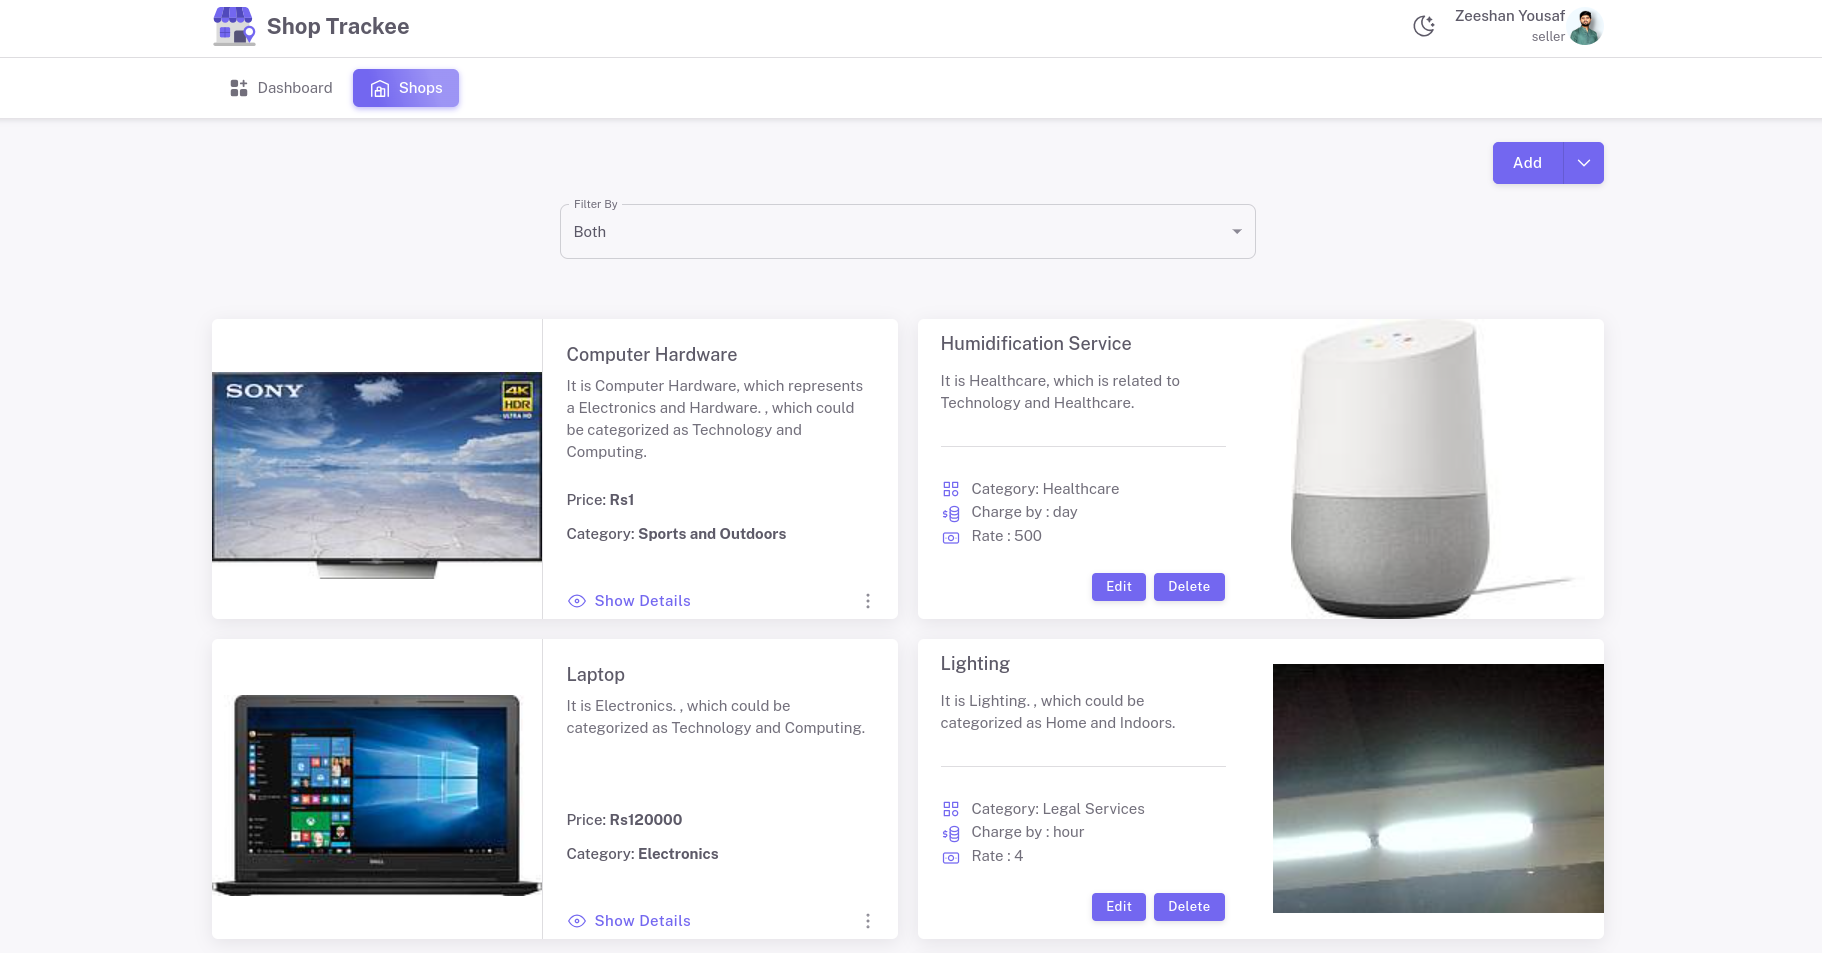
\includegraphics[width=1\textwidth]{products-services-page}
	\caption{Shop Trackee - Products and Services Listing}
\end{figure}


\begin{figure}[h]
	\subsection{Customer Home}
	\centering
	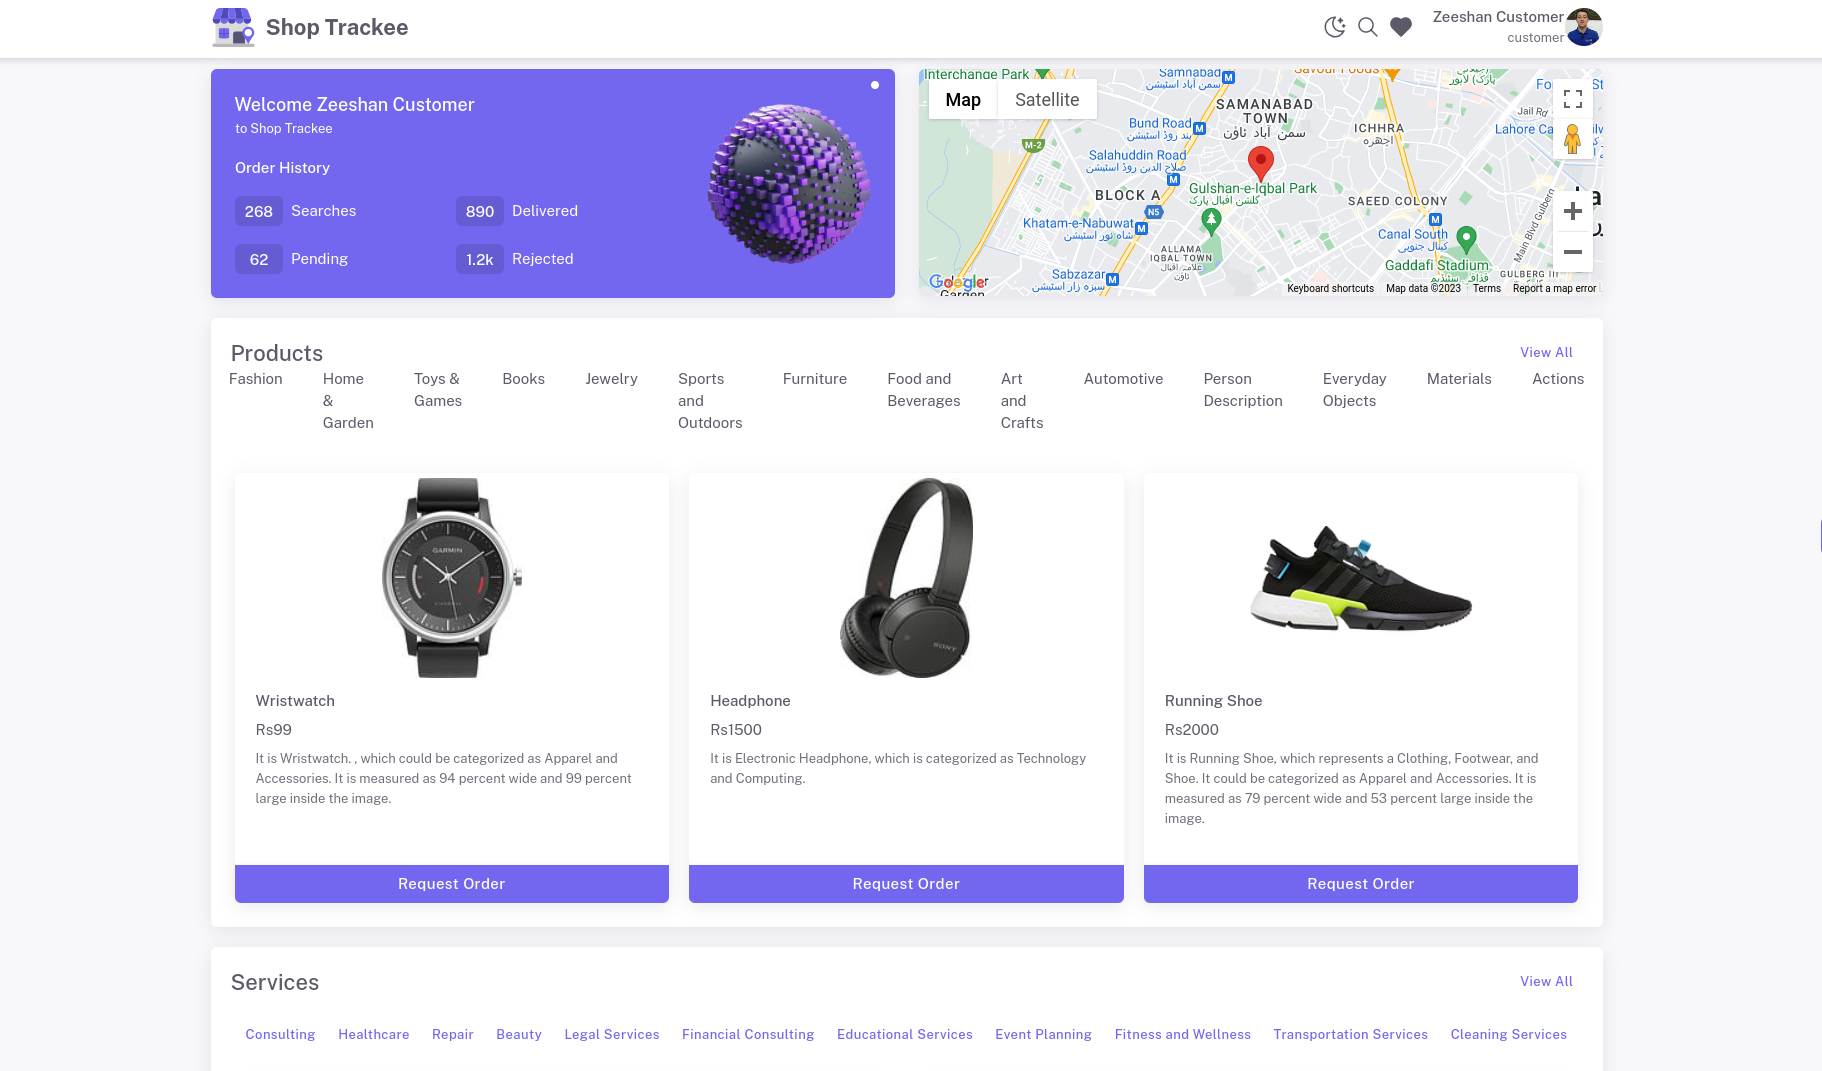
\includegraphics[width=1\textwidth]{customer-home-page}
	\caption{Shop Trackee - Customer Home}
\end{figure}
\newpage

\begin{figure}[h]
	\subsection{Customer Searching Around}
	\centering
	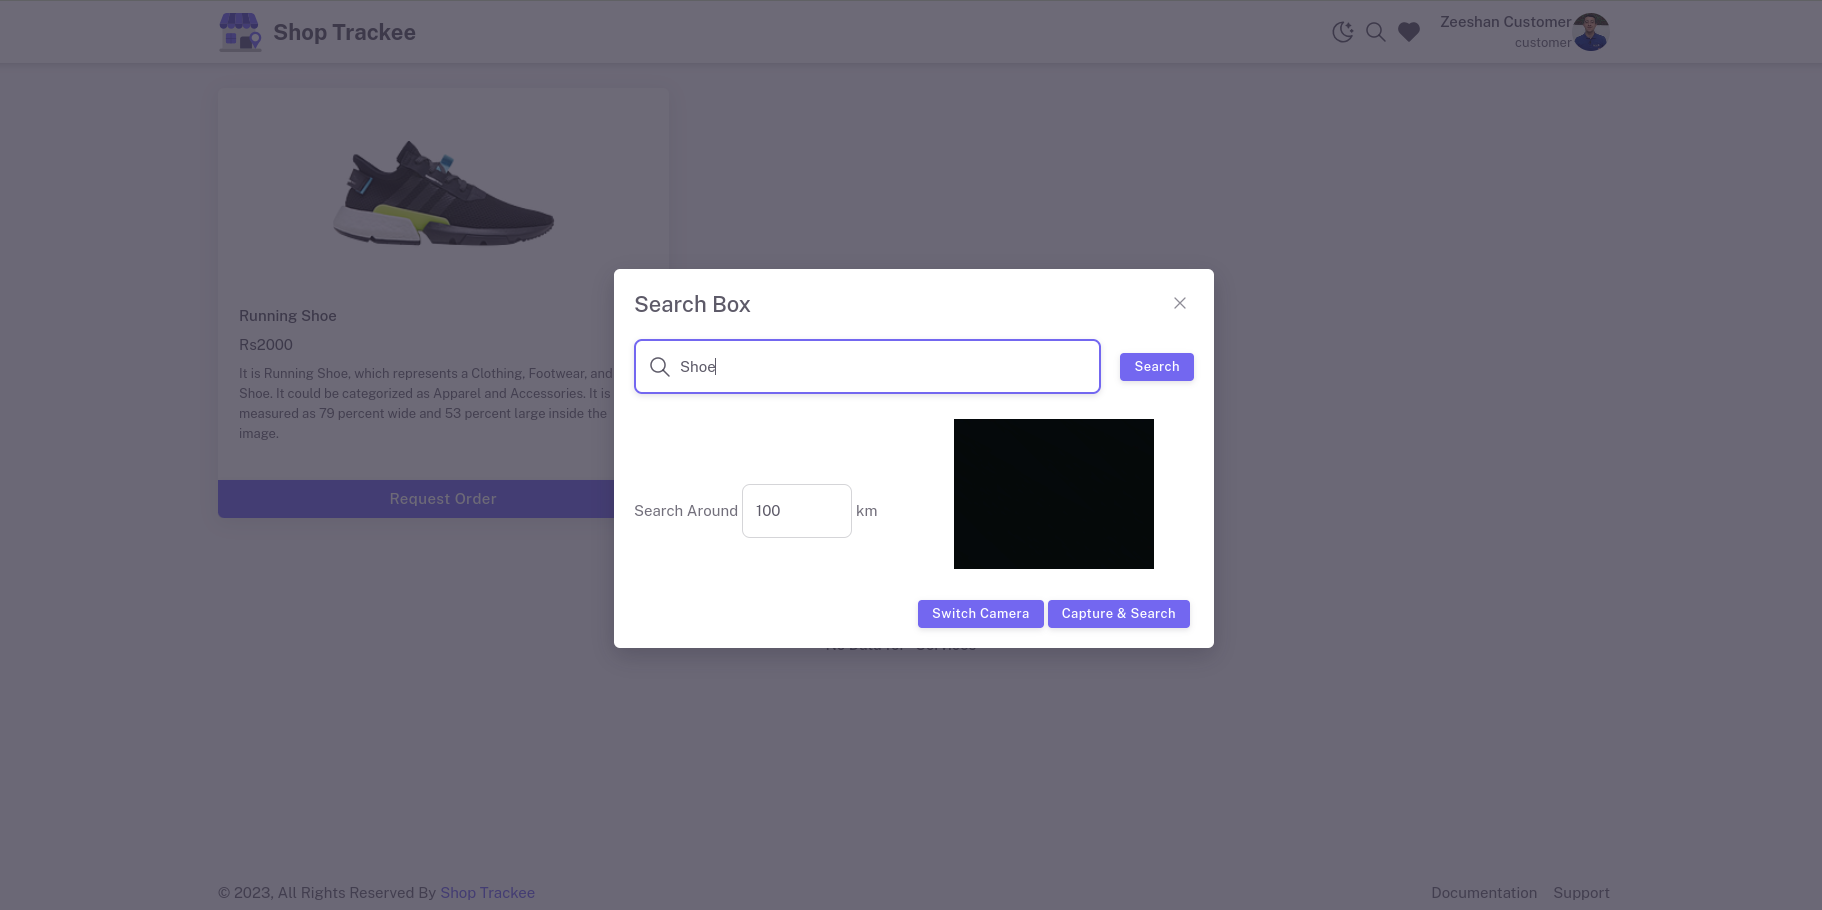
\includegraphics[width=1\textwidth]{searching-page}
	\caption{Shop Trackee - Customer Searching Around}
\end{figure}


\begin{figure}[h]
	\subsection{Customer Requesting Order}
	\centering
	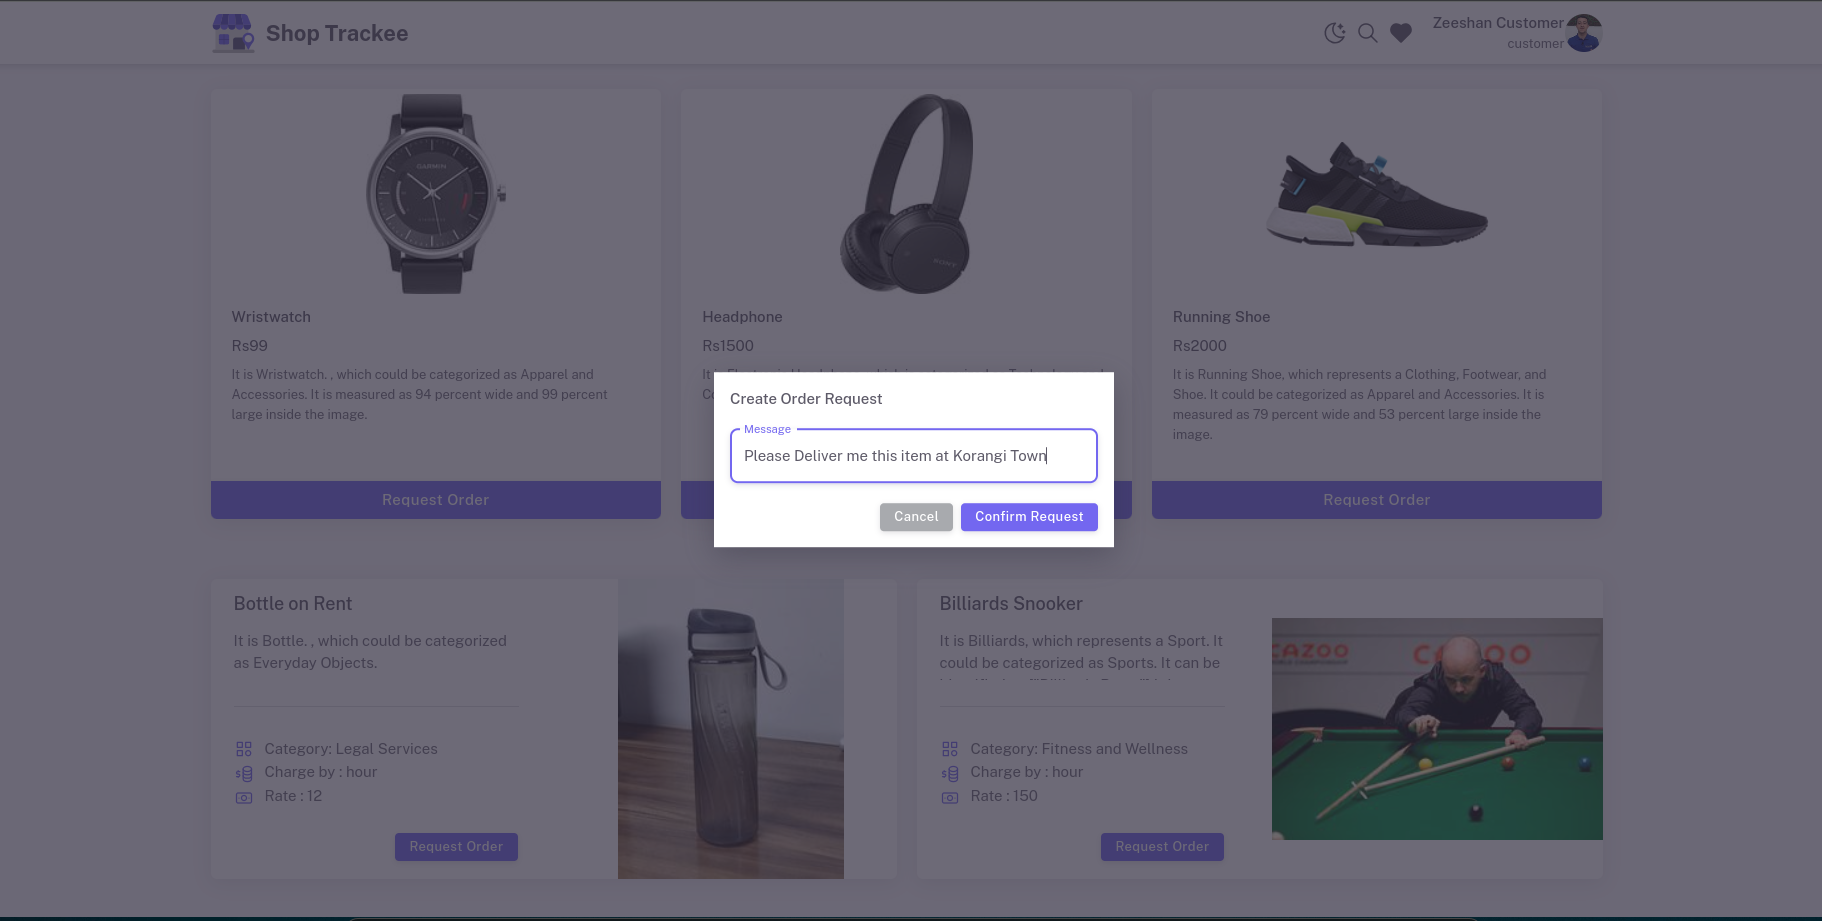
\includegraphics[width=1\textwidth]{requesting-order-page}
	\caption{Shop Trackee - Customer Requesting Order}
\end{figure}
\newpage

\begin{figure}[h]
	\subsection{Customer Order Requests History}
	\centering
	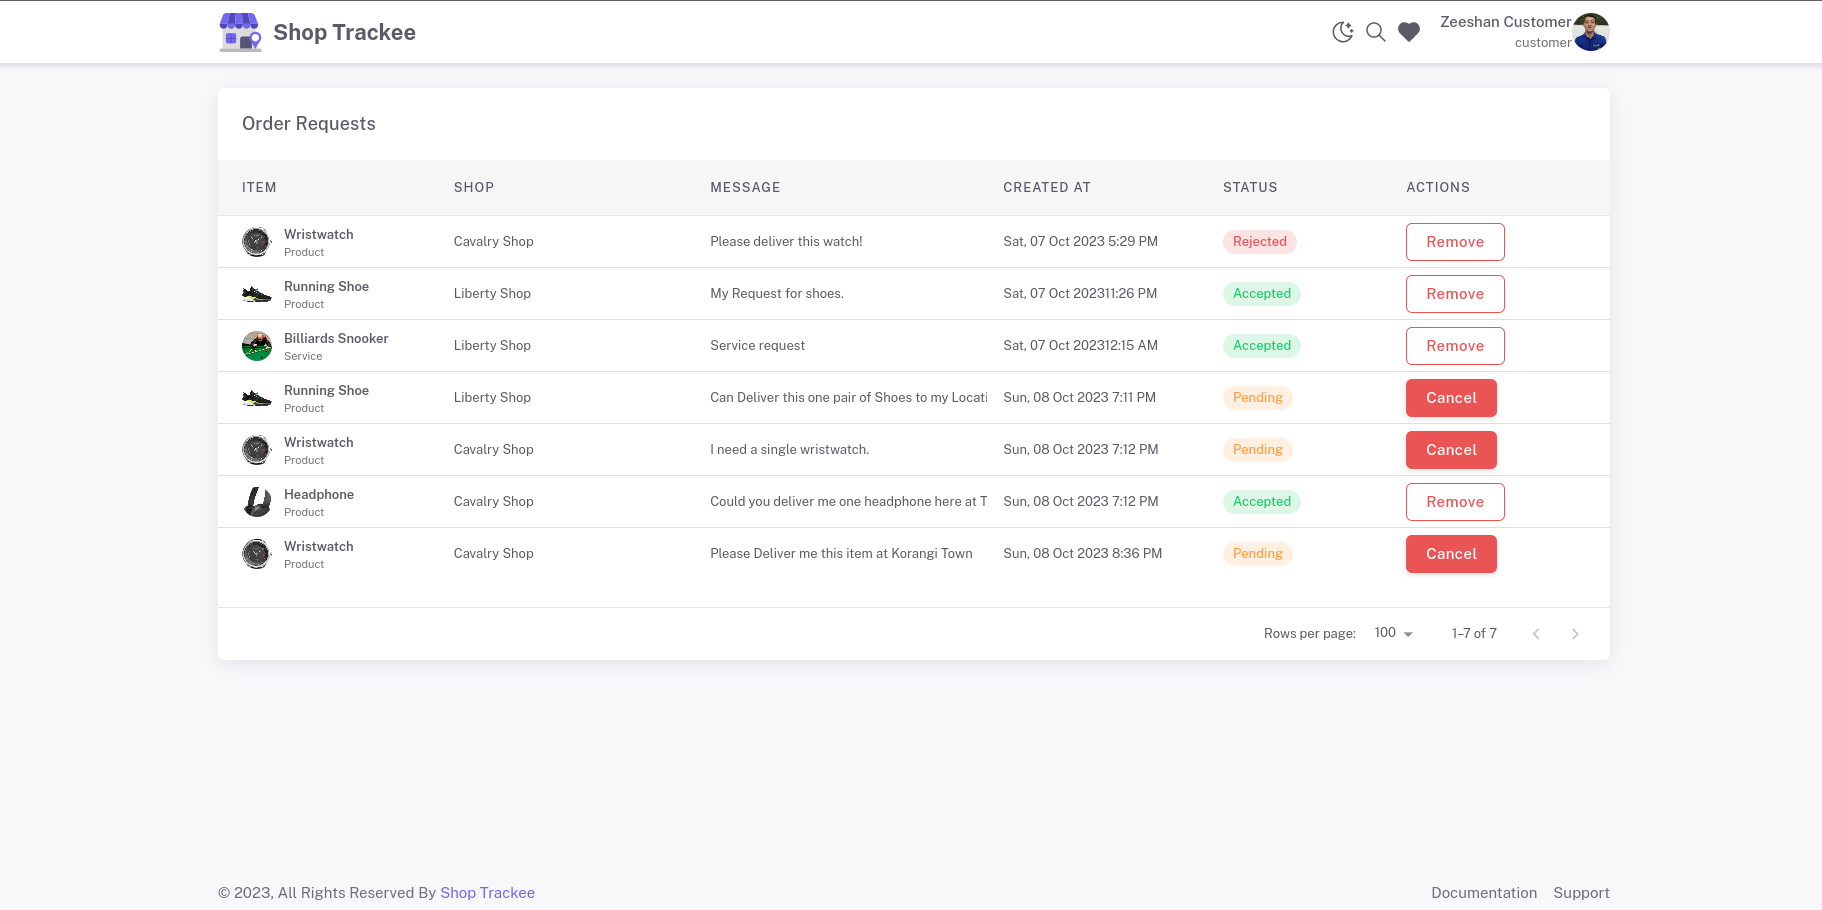
\includegraphics[width=1\textwidth]{customer-order-requests-page}
	\caption{Shop Trackee - Customer Order Requests History}
\end{figure}

\begin{figure}[h]
	\subsection{Customer Favorites}
	\centering
	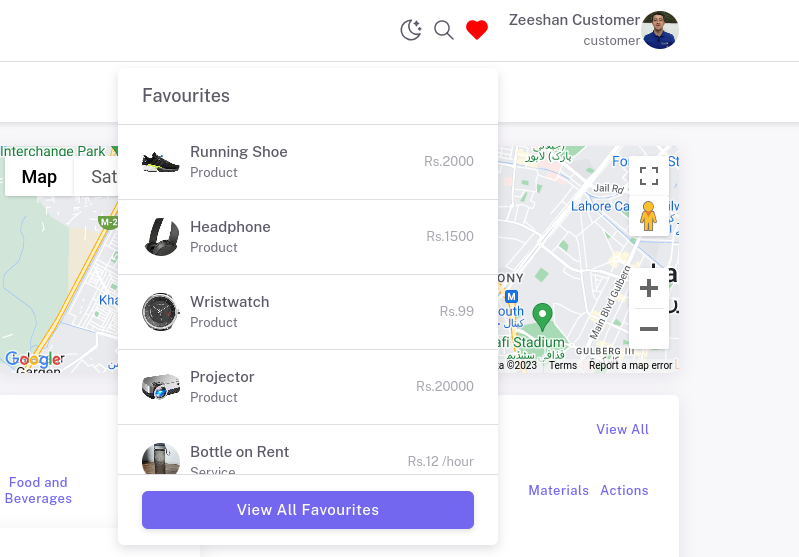
\includegraphics[width=1\textwidth]{customer-home-favorites-page}
	\caption{Shop Trackee - Customer Favorites}
\end{figure}
\newpage

\begin{figure}[h]
	\subsection{Dark Mode}
	\centering
	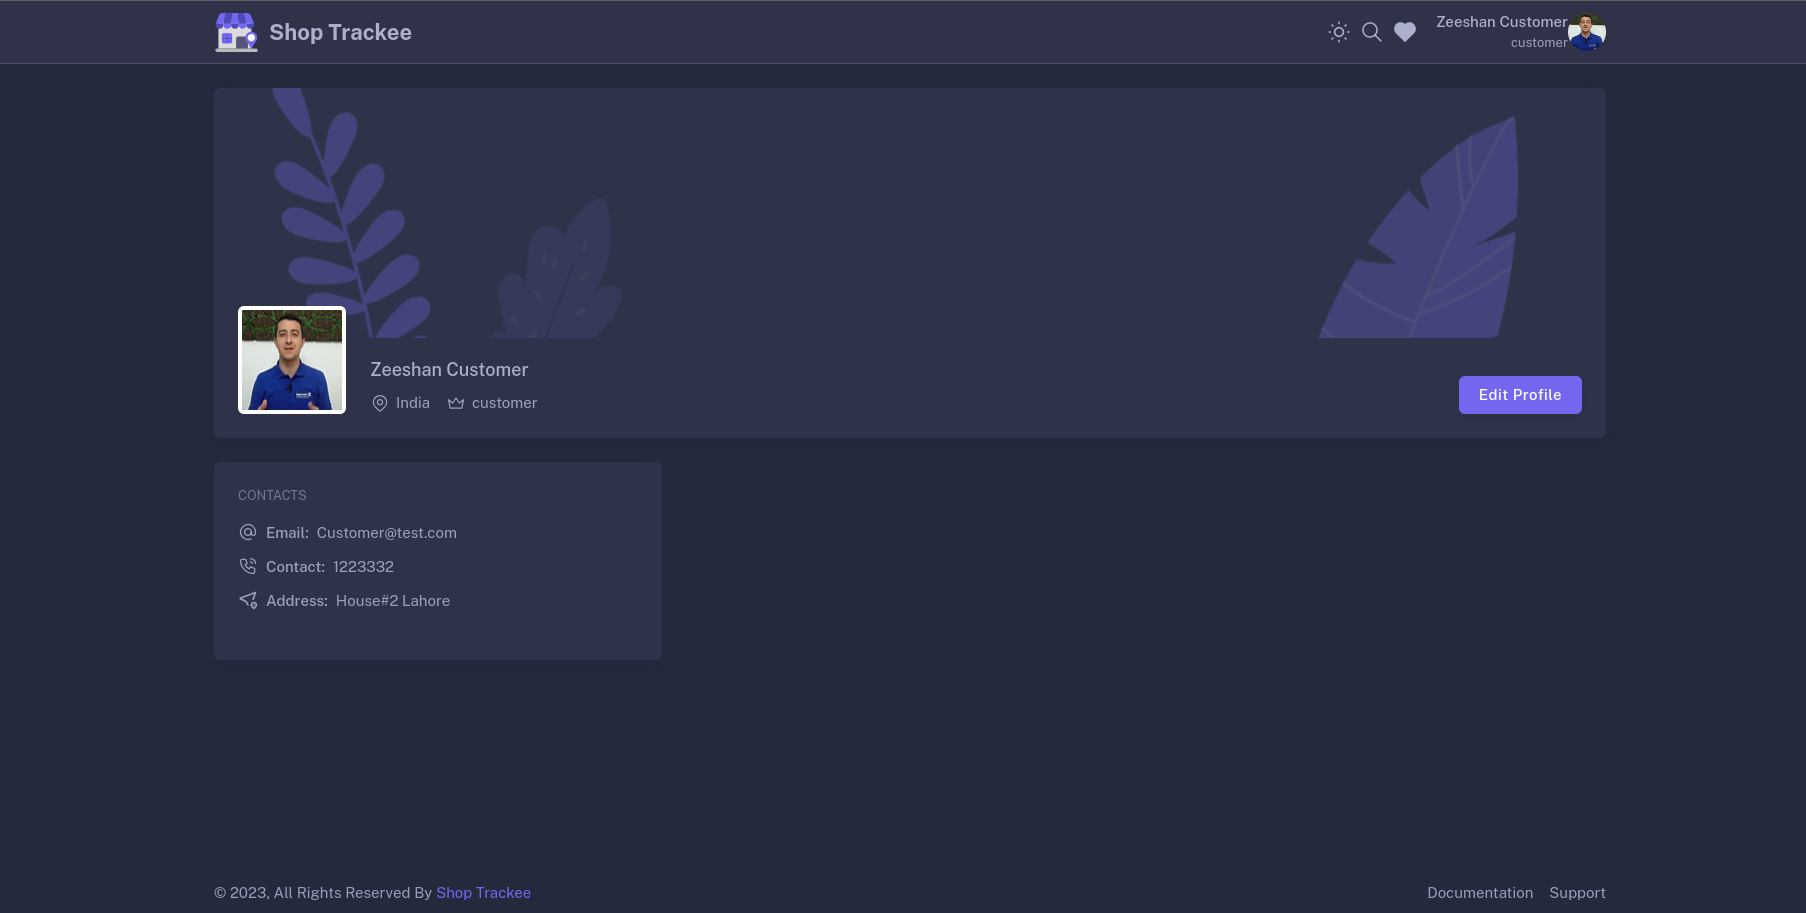
\includegraphics[width=1\textwidth]{dark-mode-profile-page}
	\caption{Shop Trackee - Dark Mode}
\end{figure}

\section{Hardware Interface}
The "Track My Shop" web application is primarily a software-based system that relies on internet connectivity and web browsers to function. However, there are a few essential hardware components and interfaces that enable its operation:

\begin{itemize}
	\item Computer Systems (Desktops, Laptops, Tablets)
	\item Smartphones and Mobile Devices
	\item Stable Internet Connection
	\item Cameras (for Image Capture)
	\item Global Positioning System (GPS) and Location Services
	\item Input Devices (Keyboards, Mouse, Touchscreens)
\end{itemize}

\subsection{Requirements}
Here are some minimal requirements of hardware to run this Web Application:
\begin{itemize}
	\item Pentium 4 - 1.9Ghz  
	\item RAM 1 GB+ 
	\item System Storage (minimum 1 GB)
	\item Windows, Linux, Mac, Andriod, IOS
	\item Browsers (Chrome 64+, Edge 79+, Firefox 67+, Opera 51+, Safari 12+)
	\item GPS WGS 84 (World Geodetic System 1984) datum for Google Maps 
\end{itemize}



\section{Evaluation}
\section{Unit Testing}
\section{Functional Testing}
\subsection{Testing Requirements}
\section{Requirements}
\newpage
\begin{center}
 \textbf{ Some more samples of tables}
\end{center}
Another sample for Table \\ \\
\begin{tabular}{ |p{12cm}| }
 \hline
  \textbf{Algorithm 1:} Group-TS  \\ \hline
\textbf{ Input:} Transition system of each member \{$T_1$, $T_2$, $T_3$\}. \\
  \textbf{Output:} Combined Transition System of members that is \textbf{T}.
  \begin{enumerate}
    \item Let m = 1, 2, 3
    \item $q^0_T$ = $q^0_m$.
    \item recursive search on \textbf{T} starting from initial state ($q^0_T$).
    \item $q_m$ $\in$ q.
    \item The transition of $T_m$ is defined as $\rightarrow_m$. where $\rightarrow_m$ = (q,q')
    \item $\tau$ : set of possible transitions and $\rightarrow_m$ $\in$ $\tau$ then do.
    \item $\omega$ = minimum weight of $\rightarrow_m$ when the robot finds some region.
    \item Find new state of transition system that is q' and if q' not exists then.
    \item Insert the state q' to \textbf{T}.
    \item Insert new transition to $\delta_T$ with assigning the weight $\omega$. where $\delta_T$ is the set of transitions.
    \item prolong search from new state q'
    \item else if there is no transition for (q,q') then
    \item Include transition that is from (q,q') to $\delta_T$ with assigning the weight $\omega$
  \end{enumerate}
 \\ \hline
\end{tabular}

\vspace{20pt}

\begin{table}[h]
\centering
\caption{\textbf{(a)} Results after running the Transition System} % title of Table\addtolength{\tabcolsep}
\addtolength{\tabcolsep}{-2pt}
\begin{tabular}{|c|c|c|c|c|c|c|c|c|} % centered columns (9 columns)
\hline %inserts double horizontal lines
$\mathbb{T}$ & 0 & 2 & 3 & 4 & 6 & 8 & 10 & \dots \\  [2ex] % inserts table
%heading
\hline % inserts single horizontal line
$r*_{group}$ & $q_0$,$q_0$,$q_0$ & $q_1$,$q_1$,$q_1$ & $q_1$$q_0$1,$q_2$,$q_3$ & $q_0$,$q_1$,$q_2$ & $q_1$,$q_0$,$q_3$ & $q_0$,$q_1$,$q_2$ & $q_1$,$q_0$,$q_3$ & \dots \\ [2ex] % inserting body of the table
$L_T$(.) & . & $p_1$,$p_2$,$p_4$,$\sigma$ & $p_3$,$p_5$ & $p_2$,$p_6$,$\sigma$ & $p_1$,$p_5$,$\sigma$ & $p_2$,$p_6$,$\sigma$ & $p_1$,$p_5$,$\sigma$ & \dots \\ [1.5ex]
$r_1$* & $q_0$ & $q_1$ & . & $q_0$ & $q_1$ & $q_0$ & $q_1$ & \dots \\ [2ex]
$r_2$* & $q_0$ & $q_1$ & $q_2$ & $q_1$ & $q_0$ & $q_1$ & $q_0$ & \dots \\ [2ex]
$r_3$* & $q_0$ & $q_1$ & $q_3$ & $q_1$ & $q_0$ & $q_1$ & $q_0$ & \dots \\ [2ex] % [1ex] adds vertical space
\hline %inserts single line
\end{tabular}
\label{table:nonlin} % is used to refer this table in the text
\end{table}

We assume in Table 4.1 the first row shows the time when the transition occur, second row represents the run $r*_{group}$, third row corresponds to the satisfied propositions, and last three rows shows the separate run of these three robots. We observed in the optimal run that ($q_0$,$q_0$,$q_0$), ($q_1$,$q_1$,$q_1$), ($q_1$$q_0$1,$q_2$,$q_3$) is prefix and ($q_0$,$q_1$,$q_2$), ($q_1$,$q_0$,$q_3$) is suffix cycle and that will be repeated an infinite number of times. The given time which satisfies the $\sigma$ is $\mathbb{T^\sigma}$ = \{2,4,6,8,10,\dots\} and the function defined in (3.2) is $C(\mathbb{T})$ = 2.

Now, the time sequence when $\sigma$ is repeatedly satisfied is $\mathbb{T^\sigma}$ = \{2,4,6,8,10,\dots\} and cost function is given as;

 \hspace{30pt}  $C(\mathbb{T})$ = $\lim_{k\to+\infty}$ ($\mathbb{T}$(k+1) - $\mathbb{T}$(k))

\hspace{30pt}  = $\mathbb{T}$(k+1) - $\mathbb{T}$(k)

\hspace{30pt}  = 4 - 2 = 2

 As $C(\mathbb{T})$ = 2 is the obtained function where the $\sigma$ is repeatedly satisfied. At t=3, robot2 has reached at $q_2$ while the robot1 is still moving from $q_1$ to $q_0$, therefore $r_1$* has no correlated state to t=3.

 \subsection{Accurate Specified Run}
 In Algorithm.2 the exact solution is summarized and it shows that a particular solution is given to a specified problem for that case where robots have exact time information.

\begin{center}
\begin{tabular}{ |p{12cm}| }
 \hline
 \textbf{Algorithm 2:} Accurate-Run \\ \hline
\textbf{ Input:} \{$T_1$,$T_2$, $T_3$\} \& LTL formula $\phi$. \\
  \textbf{Result:} Different runs of each system in the form \{$r_1$*,$r_2$*,$r_3$*\} that satisfies $\phi$.
  \begin{enumerate}
    \item n = 1, 2, 3
    \item Model the group transition system \textbf{T}.
    \item Now search runs $r*_{group}$ for the system as done in Table.1.
    \item Trace runs $r*_{group}$ on the transition systems $T_n$ to obtain the runs $r_n$*.
    \item Then find obtained function where $\sigma$ is satisfied.
  \end{enumerate}
 \\
 \hline
\end{tabular}
\end{center}

As the grouped transition system \textbf{T} is constructed by using Algorithm.1 to model the team. After that we obtain a run $r*_{group}$ on \textbf{T} that satisfies the LTL formula.

\vspace{10pt}
\begin{table}[h]
\centering
\caption{\textbf{(b)} Results after running the Transition System} % title of Table
\addtolength{\tabcolsep}{-6pt}
\small
\begin{tabular}{|c|c|c|c|c|c|c|c|c|c|c|} % centered columns (9 columns)
\hline %inserts double horizontal lines
$\mathbb{T}$ & 0 & 2 & 3 & 4 & 5 & 6 & 7 & 8 & 9 & \dots \\  [2ex] % inserts table
%heading
\hline % inserts single horizontal line
$r*_{group}$ & $q_0$,$q_0$,$q_0$ & $q_1$,$q_1$,$q_1$ & $q_1$$q_0$1,$q_2$,$q_3$ & $q_0$,$q_1$,$q_2$ & $q_0$$q_1$1,$q_2$,$q_3$ & $q_1$,$q_1$,$q_1$ & $q_1$$q_0$1,$q_2$,$q_3$ & $q_0$,$q_1$,$q_2$ & $q_0$$q_1$1,$q_2$,$q_3$ & \dots \\ [2ex] % inserting body of the table
$L_T$(.) & . & $p_1$,$p_2$,$p_4$,$\sigma$ & $p_3$,$p_5$ & $p_2$,$p_6$,$\sigma$ & $p_3$,$p_5$ & $p_1$,$p_2$,$p_4$,$\sigma$ & $p_3$,$p_5$ & $p_2$,$p_6$,$\sigma$ & $p_3$,$p_5$ & \dots \\ [2ex]
$r_1$* & $q_0$ & $q_1$ & . & $q_0$ & . & $q_1$ & . & $q_0$ & . & \dots \\ [2ex]
$r_2$* & $q_0$ & $q_1$ & $q_2$ & $q_1$ & $q_2$ & $q_1$ & $q_2$ & $q_1$ & $q_2$ & \dots \\ [2ex]
$r_3$* & $q_0$ & $q_1$ & $q_3$ & $q_1$ & $q_3$ & $q_1$ & $q_3$ & $q_1$ & $q_3$ & \dots \\ [2ex] % [1ex] adds vertical space
\hline %inserts single line
\end{tabular}
\label{table:nonlin} % is used to refer this table in the text
\end{table}

\vspace{10pt}
Now similarly in Table 4.2 the first row shows the time when the transition occur, second row represents the run $r*_{group}$, third row corresponds to the satisfied propositions, and last three rows shows the separate run of three robots. As we observed in the optimal run that ($q_0$,$q_0$,$q_0$), ($q_1$,$q_1$,$q_1$) is the prefix and ($q_1$$q_0$1,$q_2$,$q_3$), ($q_0$,$q_1$,$q_2$), ($q_0$$q_1$1,$q_2$,$q_3$), ($q_1$,$q_1$,$q_1$) is the suffix cycle and that will be repeated an infinite number of times. The given time which satisfies the $\sigma$ is $\mathbb{T^\sigma}$ = \{2,4,6,8,10,\dots\} and the function defined in (3.2) is $C(\mathbb{T})$ = 2.

Now as we done in Table 4.1 similarly the same procedure for this run shown in Table 4.2, the time sequence when $\sigma$ is repeatedly satisfied is $\mathbb{T^\sigma}$ = \{2,4,6,8,10,\dots\} and cost function is given as;

\hspace{30pt}  $C(\mathbb{T})$ = $\lim_{k\to+\infty}$ ($\mathbb{T}$(k+1) - $\mathbb{T}$(k))

\hspace{30pt}  = $\mathbb{T}$(k+1) - $\mathbb{T}$(k)

\hspace{30pt}  = 4 - 2 = 2

 As $C(\mathbb{T})$ = 2 is the obtained function where the $\sigma$ is repeatedly satisfied.

 For some applications including new states and corresponding transitions to the structure of the robotic system may indicate to introducing advance stages or motion commands at some lower level. So the proper way in which the changes of these models are strictly application specific and we do not consider such details in our work. Assuming that these changes can be implemented in future.

 \subsection{Synchronized Specification}
 If there is a situation in which robots are moving at uncertain time and $\phi$ is not satisfied then we consider individual synchronization run for the robots that helps in guarantee the correctness of the model. In Algorithm.3 the protocols which is followed by the robots for synchronization in the field.

 \begin{center}
\begin{tabular}{ |p{13cm}| }
 \hline
 \textbf{Algorithm 3:} Synchronized-Move \\ \hline
\textbf{ Input:} $r_i$ and sequence $s_i$ of $robot_i$ \\
  \textbf{Result:} Simple synchronized moves for each robot that satisfies $\phi$.
  \begin{itemize}
    \item Initialized z at 0 and while True do
  \end{itemize}
    \begin{enumerate}
    \item report all the members.
    \item wait until all members received their information message.
    \item after satisfying propositions at $r_i^{z}$ create a transition to $r_i^{z+1}$.
    \item z = z+1.
  \end{enumerate}
 \\
 \hline
\end{tabular}
\end{center}


